\documentclass[runningheads,a4paper]{llncs}

\usepackage[T1]{fontenc}
\usepackage{lmodern}
\usepackage{graphicx}
\usepackage{amsmath}
\usepackage{marvosym}

\begin{document}

\title{Beyond Student Labels: Evaluating Prompt Sensitivity in AI-Generated Practice Problems for Multilingual Learners}
\titlerunning{Beyond Student Labels}

\author{Satyanarayana Rudraraju\textsuperscript{(\Letter)}}
\authorrunning{S. Rudraraju}

\institute{Whitney M. Young Magnet High School, Chicago, IL, USA \\ \email{rudrarajumc@gmail.com}}

\maketitle

\begin{abstract}
Tutoring multilingual students in Hyderabad, India, I noticed that telling an AI a student was learning English seemed to produce easier practice problems, in the mathematics and not only the wording. I tested this in a fully-crossed experiment (three ability levels, four language descriptions, three prompt wordings, five topics) on three free, open-weight models (Llama 3.3 70B, GPT-OSS-120B, Mistral Small), collecting 1{,}620 generations. Averaged over ability levels and Holm-corrected, an ELL-Mandarin label cut solution steps by 0.65 and operations by 4.24 (both corrected $p<.001$) and an ELL-Spanish label cut steps by 0.52 (corrected $p=.007$). Averaging departs from my pre-specified model, whose coefficients give the on-level effect, which is null. A generic ``multilingual'' label left steps unchanged, and an explicit ``struggling with this topic'' label moved them by $-0.01$ ($p=.91$). Three bounds apply: steps and operations are read from the model's own solution, so they index solution length, not intrinsic difficulty, and the effect shrinks by half or more among problems whose answer key is correct; the effect was significant in two model families and not detected in the third; and the ELL-Spanish effect cannot be separated from language switching. Models also switched languages unprompted (50.4\% of ELL-Spanish problems came back in Spanish), and exact arithmetic confirmed wrong answer keys in 13 of 14 Llama and 14 of 27 Mistral audited rational-number items, against 0 of 28 for GPT-OSS.

\keywords{Large language models \and Algorithmic fairness \and Multilingual learners \and Prompt sensitivity \and LLM-as-judge.}
\end{abstract}

\section{Introduction}

This study grew out of a free tutoring program I run in Hyderabad, India, for multilingual students who study math in English while speaking Telugu at home. When I told a large language model a student was learning English, the problems came back easier. The wording was simpler, which I expected; the mathematics looked simpler too, which I did not. This paper tests that impression.

The concern has roots in education research. Teacher expectations can shape student performance \cite{rosenthal1968} and stereotypes about a group can lower its members' performance \cite{steele1995}, though the size of both effects is debated. English-language-learner (ELL) classification lowers teachers' perceptions of a student's academic skills independent of ability \cite{umansky2021}, and tracking research documents a similar dynamic with curricular material \cite{oakes1985}. Separately, linguistic complexity in test items depresses ELL students' measured math performance \cite{abedi2001}. An ELL label describes English proficiency, not mathematical ability, and an AI system that treats the two as correlated would automate a documented human bias at the scale of every generated problem.

I study problem writing, not solving. Benchmarks test whether models can solve problems, in English \cite{cobbe2021} and in translation \cite{shi2022}; less is known about what they write for a described student, even as this becomes a standard tutoring-tool feature \cite{kasneci2023}. Writing is where a label can leak into content, because the model picks the numbers, operations, names, setting, and sometimes the language. I test free, open-weight models because they are what a low-budget tutoring program can actually run. The paper contributes a design that measures math and language difficulty separately under an ELL label, a comparison with an explicit ability label, a measurement of unprompted language switching, and an exact-arithmetic audit of answer keys.

\section{Related Work}

A described identity changes a model's outputs and can degrade performance for some groups \cite{gupta2023}; audits find demographic details push generations toward stereotypes \cite{deshpande2023,sheng2019}, with effects that differ across models \cite{gallegos2024}, and chatbots let a revealed identity shift their recommendations \cite{kantharuban2025}. Blodgett et al.\ ask that bias claims state their normative grounding \cite{blodgett2020}; mine is that a language label should change language, not mathematics.

On generation, MATHWELL \cite{christ2024} has teachers rate model-written word problems and finds that existing models often fail to be educationally appropriate. Related work covers multilingual generation \cite{gamage2025,niyarepola2022} and deliberate localization of names and settings \cite{azime2026}, close to what I observe happening unrequested. A 2026 systematic review proposes a framework for evaluating the quality of generated problems \cite{utami2026}, and models are sensitive to meaning-preserving changes in prompt format \cite{sclar2023}. Marchisio et al.\ \cite{marchisio2024} document ``language confusion'', models answering in a language the user did not ask for, and find Llama and Mistral models especially prone to it, more so at higher sampling temperatures; the same two families switch most here (Sect.~\ref{sec:h5}). LLM judges agree well with humans in aggregate but show position, length and same-family biases \cite{zheng2023}, so I use cross-family judging with a human check. The closest prior work is Weissburg et al.\ \cite{weissburg2025}, who show that LLMs acting as ``teachers'' generate and select educational content differently across race, gender, income, disability and national origin. That narrows what is new here to two things their study does not do: it tests a language-proficiency label, and it measures the mathematics of a generated problem separately from its wording.

\section{Method}\label{sec:method}

\subsection{Design}\label{sec:design}

Five hypotheses were written down in \texttt{DESIGN.md}, dated 2026-07-03 but first committed publicly on 2026-08-06, after data collection. With no external timestamp it is an analysis plan, not an independently registered protocol, and I call it ``pre-specified'' for that reason. H1 (manipulation check): math difficulty rises with stated ability. H2 (headline): ELL labels lower math difficulty versus a no-mention control. H3: ELL labels lower language difficulty. H4: effects vary ($|\Delta|>0.2$ SD) across reworded prompts. H5: language-specific labels change names and settings (only names were analysed). Fair adaptation is H3 without H2.

The design is fully crossed: three ability levels (struggling, on-level, advanced) $\times$ four language descriptions (control, multilingual, ELL-Spanish, ELL-Mandarin) $\times$ three prompt wordings $\times$ five 7th-grade topics (proportions, percents, two-step equations, rational operations, circles) $\times$ three repeats at temperature 0.7, giving 540 generations per model and $N=1{,}620$. The language description is a clause appended to an otherwise identical English prompt; control appends nothing. Where control reads ``...for a 7th-grade student who is struggling with this topic,'' ELL-Spanish adds ``...and is an English language learner whose first language is Spanish'' and multilingual adds ``...and is a multilingual learner.'' The ELL labels thus differ from the multilingual label both in the phrase ``English language learner'' and in naming a language. Before correction, pooled power is $\approx.80$ for $d=0.2$; within one model it is only $\approx.67$ for $d=0.3$, below what \texttt{DESIGN.md} claimed.

The models were Llama 3.3 70B (via Groq), GPT-OSS-120B (via Cerebras) and Mistral Small (the floating alias \texttt{mistral-small-latest}), all on free tiers, collected 2026-07-03 to 2026-07-07. Gemini was dropped: its quota allowed 138 of 540 requests (114 to 2.5 Flash, 24 to 2.5 Flash-Lite), and only 29 responses parsed; the other 109 were cut off by my 1{,}024-token output cap.

\subsection{Measures}\label{sec:measures}

\emph{Math difficulty.} Solution steps is the number of entries in the solution-step list the model returns. Operations is the number of arithmetic symbols in those steps, counting equals signs, every minus sign and fraction slash, and the words plus, minus, times and divided. Largest number is the largest number in the problem statement, the only problem-side measure. \emph{Language difficulty.} Flesch-Kincaid grade \cite{kincaid1975} on English output, with sentence segmentation that ignores decimal points. Output language is classified by a deterministic rule: Chinese if more than 20\% of characters are Han, otherwise Spanish if Spanish stopwords outnumber English ones, otherwise English. It replaced \texttt{langdetect}, which had labelled 152 English problems as other languages. The rule is binary, though some outputs are bilingual (29 of GPT-OSS's 135 ELL-Spanish problems contain some Spanish).

A judge from a different model family than the writer (GPT-OSS for Llama and Mistral problems, Mistral for GPT-OSS problems) scored each problem 1--5 on correctness, difficulty fit, clarity, pedagogical soundness and cultural neutrality, and extracted character names. I rated a stratified 56-item sample (28 GPT-OSS, 28 Mistral) without seeing condition labels, although output language reveals the condition for switched items. The pre-specified bar for treating judge scores as confirmatory, Spearman $\rho\geq0.5$ on correctness and difficulty, was not fully met (Sect.~\ref{sec:judge}), so all judge-derived quantities are descriptive.

\subsection{Analysis and Departures from the Plan}\label{sec:analysis}

Each outcome is regressed on ability level, language, prompt wording, topic and model family with HC3 robust standard errors \cite{mackinnon1985}. I report each label's effect versus control averaged over ability levels, its 95\% CI, and Cohen's $d$ \cite{cohen1988} (the coefficient over the outcome SD), with Holm correction \cite{holm1979} across the nine primary tests (three math outcomes $\times$ three labels).

Averaging is the most consequential departure from the plan. \texttt{DESIGN.md} specifies ability level interacted with language and asks for the language coefficients, which with on-level as reference estimate the effect for on-level students only. That effect is null (ELL-Mandarin $-0.10$ steps, $p=.59$), and the reviewed version of this paper reported it as the result. I now take the averaged effect to be what H2 is about. A reader who holds to the plan as written should read the pre-specified test as null and the averaged estimates as a departure; both are reproducible from the study data.

\texttt{DESIGN.md} records three dated amendments (judge rotation reassigned for quota, language detection added, Gemini dropped). Not recorded there: GPT-OSS-120B replaced a retired Qwen model on 2026-07-04, before any usable data existed in that slot, and the design table was edited in place to list it; the two planned parse retries were not implemented; \texttt{langdetect} was replaced; and human validation covered 56 items from two families, not the planned 120.

\emph{AI tool use.} I used Claude (Anthropic) for drafting and revision, code review, and an audit of the statistical analysis. The audit produced the script \texttt{reanalysis.py}, which generates every statistic and figure reported here. I designed the study, collected and rated the data, and am responsible for the analysis and its interpretation.

\section{Results}\label{sec:results}

Of 1{,}620 generations, 1{,}567 (96.7\%) produced readable JSON, independent of language condition ($\chi^2=3.34$, $p=.34$).

\subsection{H1: Manipulation Check}\label{sec:h1}

An advanced label, worded ``advanced and ready for a challenge,'' raised solution steps by 1.19, operations by 7.04 and the largest number by 115.0 (all $p<.001$) versus on-level. The struggling label, which unlike the advanced one does not ask for a change in difficulty, lowered nothing (steps $p=.91$; operations $p=.61$; largest number $p=.63$). Either the models did not write easier problems for a struggling student, or they did and these measures cannot see it, for example because an easier problem came with a more fully worked solution. The data cannot separate these readings.

\subsection{H2: ELL Labels Lowered the Math Measures}\label{sec:h2}

After correction, ELL-Mandarin cut solution steps by 0.65 (95\% CI $-0.96$ to $-0.35$; $d=-0.26$; $p=.0002$) and operations by 4.24 ($-6.15$ to $-2.33$; $d=-0.26$; $p=.0001$). ELL-Spanish cut steps by 0.52 ($-0.84$ to $-0.21$; $d=-0.21$; $p=.0067$); its operations effect ($-2.61$) did not survive correction ($p=.059$). These are small effects (Fig.~\ref{fig:forest}). The multilingual label shows no effect on steps ($-0.08$, $p=.68$; 90\% CI $-0.15$ to $0.09$ SD, inside the pre-specified $\pm0.2$ band), though its operations interval ($-0.20$ to $0.02$ SD) does not establish equivalence. Largest number moved for no label on the raw scale used in the primary tests (all $p>.16$); on a post hoc log scale all three labels lowered it, multilingual included ($p=.018$).

\begin{table}[tbp]
\caption{ELL labels are compared with an explicit statement that the student is behind, in the same regression. ``Struggling'' is contrasted with on-level, the ELL labels with the no-mention control. $p$-values are uncorrected.}
\label{tab:struggling}
\centering\small
\begin{tabular}{lccc}
\hline
Measure & ``struggling'' label & ELL-Spanish & ELL-Mandarin \\
\hline
Solution steps & $-0.01$ ($p=.91$) & $-0.52$ ($p=.0010$) & $-0.65$ ($p<.0001$) \\
Operations & $+0.34$ ($p=.61$) & $-2.61$ ($p=.0099$) & $-4.24$ ($p<.0001$) \\
$\log_{10}$(largest number) & $+0.01$ ($p=.64$) & $-0.10$ ($p=.0011$) & $-0.08$ ($p=.0075$) \\
\hline
\end{tabular}
\end{table}

In Table~\ref{tab:struggling}, saying a student is struggling moved none of these measures; saying the student is learning English moved steps under both ELL labels. On these measures a language label did more than an explicit statement that the student is behind in mathematics.

\begin{figure}[tbp]
\centering
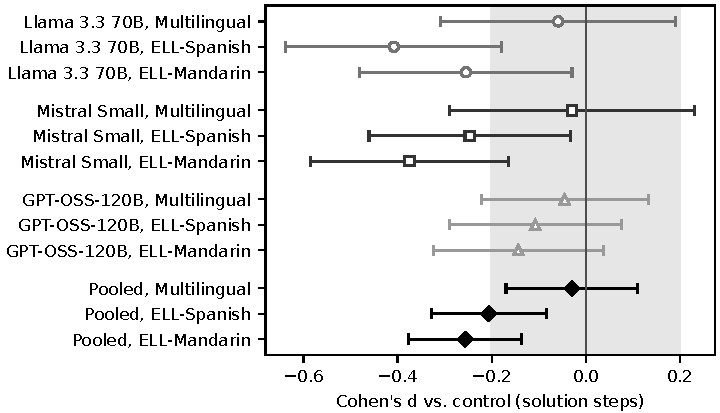
\includegraphics[width=\linewidth]{104-fig1.pdf}
\caption{The effect of each language label on solution steps is shown by model and pooled, averaged over ability levels, with 95\% confidence intervals. The shaded band is $|d|<0.2$, the equivalence band.}
\label{fig:forest}
\end{figure}

\subsection{Where the Effect Concentrates}\label{sec:where}

A pre-specified question asked whether label effects depend on stated ability. In the interacted model the level-by-language terms are jointly significant for steps ($\chi^2(6)=14.98$, $p=.020$) but not operations ($p=.14$). The simple effects, uncorrected: at on-level no ELL effect appears (ELL-Mandarin $-0.10$ steps, $p=.59$); at struggling, ELL-Mandarin removes 0.75 steps ($p=.003$); at advanced it removes 1.14 steps ($p=.001$) and 7.56 operations ($p=.001$), and ELL-Spanish 0.90 steps ($p=.014$) and 6.50 operations ($p=.008$). The drop is numerically largest for advanced students, but the advanced and struggling effects on steps do not differ significantly ($p=.37$ and $.29$), and advanced problems are longer to begin with. For ELL-Mandarin the data support an effect at both ends of the ability range and none in the middle; for ELL-Spanish, only at the advanced level (struggling $-0.42$ steps, $p=.11$). A simple ``language as a proxy for ability'' account does not predict the on-level null, and I cannot explain it.

Per model, with Holm across the nine model-by-label tests for each outcome, Llama's ELL-Spanish effect on steps ($-0.52$, $p=.0042$) and Mistral's ELL-Mandarin effect ($-1.26$, $p=.0042$) survive, as do Mistral's operation effects (ELL-Mandarin $-8.39$, $p=.0001$; ELL-Spanish $-5.68$, $p=.028$). GPT-OSS shows nothing significant, but that is not evidence of absence: its estimates point the same way, it fails the equivalence test (ELL-Mandarin steps, 90\% CI $-0.30$ to $0.01$ SD), and a model-by-label interaction test finds the families differ on operations ($p=.010$) but not reliably on steps ($p=.079$).

\subsection{H3: Language Simplification Is Uneven}\label{sec:h3}

On English output ($n=1{,}271$), ELL-Mandarin lowered Flesch-Kincaid grade by 0.77 ($p=.0003$) and multilingual by 0.42 ($p=.046$); ELL-Spanish did not ($+0.03$, $p=.94$). At the struggling level no label lowered reading grade. Pooling hides three behaviours (Fig.~\ref{fig:fk}). GPT-OSS's estimates are lower under every label (0.7 to 1.3 grades, though multilingual is $p=.07$). Mistral's English output is simpler under the multilingual and ELL-Mandarin labels. Llama does not simplify, and under ELL-Spanish its English problems are estimated more than a grade harder ($+1.20$, $p=.006$, uncorrected, $n=54$) while its steps drop by 0.52. Easier mathematics with harder English is the combination this study defined as harmful, but the evidence for it is weak: the reading estimate rests on the 43\% of Llama's ELL-Spanish problems that stayed in English, a subset conditioned on a post-treatment variable with a different topic mix (only 1 of its 26 circle problems stayed in English), and the unadjusted means differ by less (4.5 versus 4.1). The step drop is measured over all of them.

\begin{figure}[tbp]
\centering
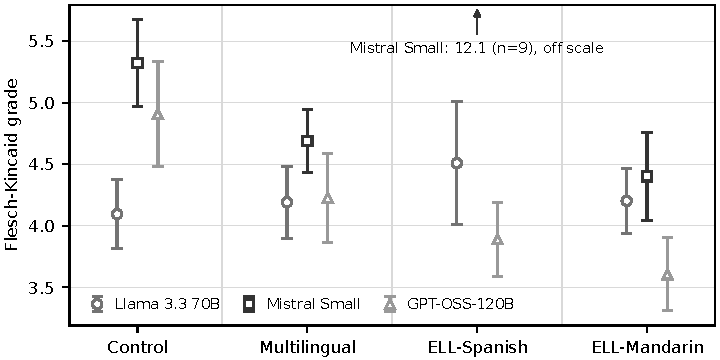
\includegraphics[width=\linewidth]{104-fig2.pdf}
\caption{Mean Flesch-Kincaid grade is shown by condition and model for English problems only, with standard-error bars. Mistral's ELL-Spanish mean (12.1) rests on 9 items and is off scale.}
\label{fig:fk}
\end{figure}

\subsection{Robustness and H4}\label{sec:robust}

With the same nine-test correction, clustering standard errors on the 539 design cells leaves ELL-Mandarin steps at $p=.0011$, its operations at $.0003$ and ELL-Spanish steps at $.028$; removing 106 near-duplicates leaves them at $.0003$, $.0002$ and $.0070$. ELL-Spanish operations stays non-significant in both ($.075$, $.095$). The step effects also survive a Poisson model ($-13\%$ and $-10\%$), winsorizing the top 1\%, median regression, a permutation test within design strata ($p\leq.001$) and the removal of any one model family (all $p<.03$, uncorrected). They are negative in 9 of the 10 label-by-topic cells, with no significant label-by-topic interaction ($p=.09$). Restricted to English-only output ($n=1{,}271$), ELL-Mandarin remains significant (steps $-0.43$, corrected $p=.037$; operations corrected $p=.042$) but the ELL-Spanish effect on steps roughly halves and is not significant even before correction ($-0.27$, $p=.14$), although its largest-number effect becomes significant ($-31.5$, corrected $p=.042$). Only 49.6\% of ELL-Spanish problems were in English, and output language is itself an effect of the label, so the ELL-Spanish effect on steps cannot be separated from the language switch that accompanies it. H4 was not supported: ranges of the pooled ELL contrast across the three wordings were 0.09 to 0.16 SD, below the 0.2 threshold, though the design is not powered to test that interaction.

\subsection{H5: Names and Language Switching}\label{sec:h5}

Character names, extracted by the judge and coded by origin after the fact, tracked the label ($\chi^2(9)=365.6$, Cram\'er's $V=0.28$). Chinese-style names appeared in 15.9\% of ELL-Mandarin problems and nowhere else. Hispanic-style names appeared in 21.8\% of ELL-Spanish problems, 0.3\% of controls, and 18.2\% of problems under the multilingual label, which names no language. The coding is rough: 53 of those 72 multilingual items rest on unaccented ``Maria''.

Models often wrote whole problems in the labelled language without being asked: 50.4\% of ELL-Spanish items came back in Spanish and 24.4\% of ELL-Mandarin in Chinese, against 0\% for control and 0.5\% for multilingual. The rate varies by model and language: for ELL-Spanish, Mistral switched 93\%, Llama 57\% and GPT-OSS 1.5\%; for ELL-Mandarin, Mistral switched 69\%, GPT-OSS 1.5\% and Llama never. This can be read as accommodation or as withholding the English mathematical vocabulary an English-medium learner needs.

\subsection{Answer Keys and Judge Validity}\label{sec:judge}

The judge flags a wrong answer key in 22.1\% of problems: 38.5\% Llama, 28.9\% Mistral, 0.4\% GPT-OSS. As an independent check I re-evaluated every problem that reduces to a pure rational-number expression with exact fractions. Llama was wrong on 13 of 14, Mistral on 14 of 27, GPT-OSS on 0 of 28, and the judge agreed on all 69. These items are not a random sample, and many are repeats (Llama's 14 contain five distinct expressions), so the audit confirms the judge where it can be checked and does not estimate an error rate. GPT-OSS's 0.4\% deserves caution, because its judge was Mistral, which gets many of its own keys wrong; it is supported by the audit and by my own ratings, which found no wrong key in 28 GPT-OSS items. ELL-labelled problems carry fewer flagged keys than controls (18.5\% and 18.8\% versus 25.8\%), though the judge's accuracy on non-English problems was not checked.

On the 56-item human sample, correctness agreement was 98.2\% ($\kappa=0.66$, $\rho=0.70$), clearing the bar on correctness. The one disagreement was a wrong key (\$20.93 for \$21.00) that the judge caught and I missed. But only 2 items were judge-flagged, where the judge's Mistral rate predicts about 8, so the sample under-represents errors. I rated every item 5 on difficulty, leaving that correlation undefined, so the two-part bar is not met. I also flagged three items as culturally stereotyped that the judge passed; on review the judge was right and I had penalised the output language.

\section{Discussion and Limitations}\label{sec:discussion}

Naming an English learner's first language shortened the solutions these models wrote by about half a step (0.21 to 0.26 SD). That is the pattern expected if a model treats a language label as information about mathematical ability, the bias documented in teachers \cite{umansky2021}, but the design does not isolate that mechanism.

The measures carry the largest caveat. Steps and operations describe how a solution is narrated as much as how hard the problem is, so a model that writes a terser solution for an English learner would score as writing easier mathematics. The one problem-side measure moves less, and it also moves under the multilingual label that leaves steps untouched. The solutions being measured are often wrong in the two families that show the effect. The output format asked for the answer before the solution steps, so Llama and Mistral commit to an answer before working the problem and, when the working disagrees, often write the correction into the steps; GPT-OSS reasons before it responds. Wrong keys are therefore partly a product of this format, and such corrections lengthen the solutions being counted. Among the 1{,}220 problems whose key the judge accepted, the ELL-Mandarin effect on steps halves ($-0.33$, $p=.008$) and the ELL-Spanish effect is no longer significant ($-0.19$, $p=.16$), so part of the headline effect may run through fewer wrong keys and corrections under the ELL labels. Table~\ref{tab:struggling} bears on this without settling it: if step count tracked only how much a model writes for a weaker student, the struggling label should move it, and it does not; but that null is also a failed manipulation check, and the two contrasts use different baselines. Settling intrinsic difficulty needs a fixed solver or blind teacher ratings.

Other limits follow from the design. The ELL labels differ from the multilingual label in two ways, so I cannot say whether the phrase or the named language matters. Only two languages were tested, and Telugu was not. The control appends no clause, though the multilingual label adds one and leaves steps unchanged. Each model ran on a different provider with a different output cap (3{,}000 tokens for GPT-OSS, 1{,}024 for the others), and 37 of Llama's 44 unreadable outputs were cut off by that cap, 23 at the advanced level; imputing all 40 cut-off outputs at the 90th percentile of steps for their model and level leaves both ELL effects in place ($-0.63$, $-0.53$). Flesch-Kincaid is unstable on problems two or three sentences long. The per-level and per-model reading estimates are uncorrected. The human check is one rater on 56 items, with Llama never validated, which is too little to support claims about cultural content or about problem difficulty. Personas are not students, and nothing here extends to learning outcomes or frontier models. Whether unprompted switching helps depends on facts the model is never told.

For practice: stating ability does not prevent a language label from changing the problem, so generate with and without the label and compare; do not assume English output; check the arithmetic; and choose the model first, since families differ far more on answer-key errors (0.4\% to 38.5\%) and switching into Spanish (1.5\% to 93\%) than conditions do.

\section{Conclusion}

Across 1{,}620 problems from three free models, an ELL label with a named first language shortened the written solution by about half a step, while stating that the student was behind changed nothing on the same measures. The effect was clearest at the advanced level and absent at on-level, was absent for a generic multilingual label, and was significant in two of three model families. Whether it reflects easier mathematics or terser solutions is not settled, and for ELL-Spanish it cannot be separated from the switch into Spanish. Two of the three models were judged to produce wrong answer keys on more than a quarter of their problems. Educators should compare output with and without a language label, check the arithmetic, and not assume they will get English back.

\begin{credits}
\subsubsection{Data and Code Availability.}
\begingroup\sloppy
The data, the collection and scoring code and the analysis plan (\texttt{DESIGN.md}) are public at \url{https://github.com/rudrarajumc-star/Beyond-Student-Labels-Research-Paper}; \texttt{reanalysis.py} is available from the author on request.
\par\endgroup

\subsubsection{\ackname}
No human participants or student data were used; all ``students'' are fictional prompt personas, and I provided all ratings. I received no funding.

\subsubsection{\discintname}
I declare no competing interests.
\end{credits}

\input{104.bbl}

\end{document}
